\documentclass[aspectratio=169]{beamer}


\usepackage[utf8]{inputenc}
\usepackage{amsmath}
\usepackage{amsfonts}
\usepackage{amssymb}
\usepackage{graphicx}
\usepackage{ragged2e}  % `\justifying` text
\usepackage{booktabs}  % Tables
\usepackage{tabularx}
\usepackage{tikz}      % Diagrams
\usetikzlibrary{calc, shapes, backgrounds}
\usepackage{amsmath}
\usepackage{amssymb}
\usepackage{dsfont}
\usepackage{url}       % `\url
\usepackage{listings}  % Code listings
\usepackage[T1]{fontenc}
%%%%
\usepackage[style=authortitle,backend=bibtex]{biblatex}
\addbibresource{bibliography.bib}
%%%%

\usepackage{theme/beamerthemehbrs}

\author[Jain]{Gautam Kumar Jain}
\title{End-to-End Prediction of Driving
Commands Using 3D Lane Detection as an
Auxiliary Task}
%\subtitle{Subtitle of presentation}
\institute[HBRS]{Hochschule Bonn-Rhein-Sieg}
\date{\today}
\subject{Test beamer}

% leave the value of this argument empty if the advisors
% should not be included on the title slide
\def\advisors{Prof. Dr Paul G. Plöger , Prof. Dr. Sebastian Houben, Prof. Dr. Arun K. Singh}

%\thirdpartylogo{images/uni_tartu_logo.png}


\begin{document}
{
\begin{frame}
\titlepage
\end{frame}
}

%%%% _________ Introduction________%%%%%
\begin{frame}{Problem Statement}
    \begin{itemize}
        \item This project aims at predicting driving commands and 3D road lanes using a sequence of monocular images.
        \item The whole scenario can be seen as a multi-task learning problem.
        \item Prediction of driving commands is considered as main task and the prediction of 3D lanes is the auxiliary task.
        \item The project further aims to investigate the following: 
        \begin{itemize}
            \item Can 3D lane detection improve the prediction of driving commands? 
            \item Is the whole pipeline more interpret-able by the introduction of auxiliary task.
            \item Can multitask learning improve generalization? 
            \item Can task loss balancing favor the performance of the main task? 
        \end{itemize}
    \end{itemize}
\end{frame}
%---Motivation---%

%%%%  next frame %%%
\begin{frame}{Motivation (1/5)}
  \textbf{End-to-End Autonomous Driving}
  \begin{itemize}
    \item Research done in autonomous driving is focused on two approaches
        \begin{itemize}
            \item Modular 
            \item End-to-end 
        \end{itemize}
        
  \end{itemize}
    \begin{figure}[H]
     \centering
     
%\begin{subfigure}{\textwidth}
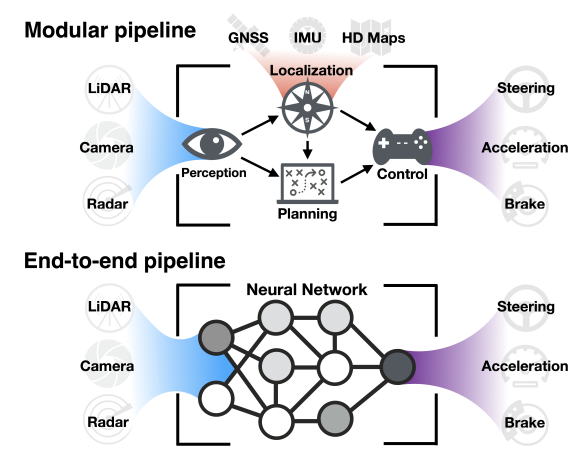
\includegraphics[width=0.4\linewidth, height=3.2cm]{images/end-modular.png} 
\label{fig:subim1}
%\end{subfigure}

\caption{Modular and end-end pipelines for autonomous driving\footcite{DBLP:journals/corr/abs-2003-06404}}
\label{fig:image2}
\end{figure}
\end{frame}

%--- Next Frame ---%
\begin{frame}{Motivation (2/5)}
  \textbf{A Driving Scenario in Autonomous Driving}
  \begin{figure}[H]
     \centering
     
%\begin{subfigure}{\textwidth}
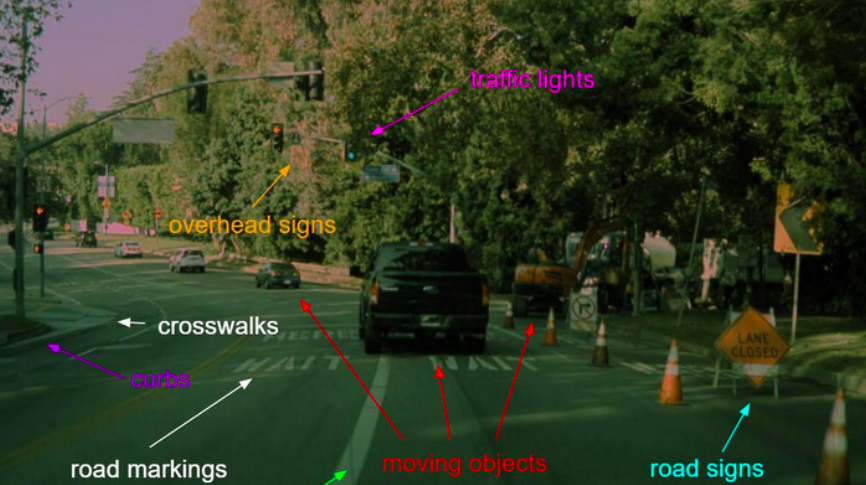
\includegraphics[width=0.6\linewidth, height=4cm]{images/MTL_aux.png} 
\label{fig:subim1}
%\end{subfigure}

\caption{Tasks to learn in a scene \footcite{tesla} }
\label{fig:image2}
\end{figure}
\end{frame}

%--- Next Frame ---%
\begin{frame}{Motivation (3/5)}
  \textbf{Multi-task Learning vs Auxiliary Learning}

  \begin{itemize}
      \item By definition, both multi-task learning and auxiliary learning is the same. 
      \item In both cases we learn for multiple tasks by the sharing the same feature representation.
      \item The difference is that in auxiliary learning we give importance to the main task while utilizing the training signals from the correlated auxiliary tasks. 
  \end{itemize}
   
\end{frame}

%--- Next Frame ---%

   
\begin{frame}{Motivation (4/5)}
  \textbf{Challenges in Multi-task Learning for End-to-End Autonomous Driving
}

  \begin{itemize}
      \item Causal confusion
      \item Distribution shift 
      \item Selection of auxiliary tasks
      \item Simulation can not cover all the scenarios 
      \item Selection of a unified feature extractor 
      \item Task loss balancing
  \end{itemize}
\end{frame}

%--- Next Frame ---%
\begin{frame}{Motivation (5/5)}
\textbf{Multi-task Learning in Autonomous Driving}
   \begin{itemize}
        \item In a driving scenario for an autonomous car to make decision we need to learn for tasks like road sign, moving objects, traffic lights and more.
        \item Generally these auxiliary tasks are correlated with the main task of prediction of driving commands.
       \item Thus learning for auxiliary tasks  along with the main task makes the driving driving policy more robust and interpret-able.
       \item Multi-task learning is an important component of the end-to-end autonomous driving.
   \end{itemize}
\end{frame}

\begin{frame}{Lane Detection in Autonomous Driving}
    \begin{itemize}
        \item In this work we have used 3D Lane detection as an auxiliary task along with the prediction of the driving commands.
    \end{itemize}
    
    \textbf{Monocular 2D Lane Detection}
    \begin{itemize}
        \item Takes an RGB image from a front facing camera mounted on autonomous vehicle and provides the set of pixels which represents lane lines. 
        \item Both input and output are represented in the image space ie. why these approaches are called 2D
        \item The basic assumption is that the ground plane is flat.
        
    \end{itemize}
    
    \textbf{Monocular 3D Lane Detection}
    \begin{itemize}
        \item In the driving scenarios where the roads are with different allevation.
        \item We need to obtain 3D points of the lanes to perform accurate motion planning.
        \item Provides real world 3D coordinates of the lane lines with respect to a camera coordinate system.
    \end{itemize}
\end{frame}
%%%%%%%%%%%%%%%%%%%
\begin{frame}{3D Lane Geometry}
    \begin{figure}[H]
     \centering
     
%\begin{subfigure}{\textwidth}
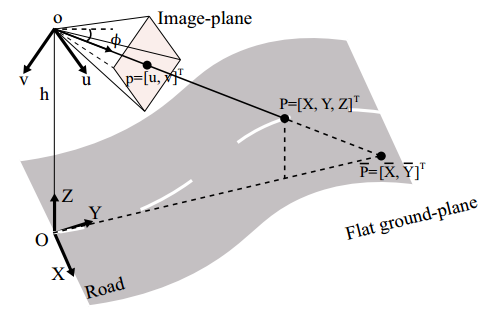
\includegraphics[width=0.6\linewidth, height=4cm]{images/3d_lane_geometry.png} 
\label{fig:subim1}
%\end{subfigure}

\caption{Geometric representation of lane point in 3D world space, image plane and virtual top view \footcite{DBLP:journals/corr/abs-2112-15351} }
\label{fig:image2}
\end{figure}
\end{frame}
% ----- next frame ------%
\begin{frame}{Inspiration for Proposed 3D Lane Detector (1/2)}
\textbf{Approach 1: Gen-LaneNet}

 \begin{figure}[H]
     \centering
     
%\begin{subfigure}{\textwidth}
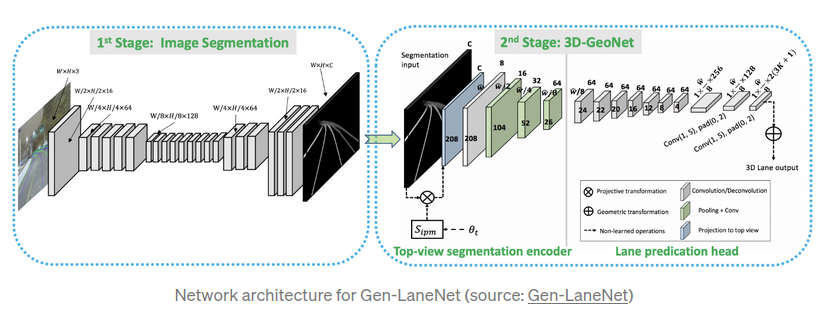
\includegraphics[width=0.8\linewidth, height=4cm]{images/genLanenet.png} 
\label{fig:subim1}
%\end{subfigure}

\caption{Gen-LaneNet pipeline \footcite{guo2020gen} }
\label{fig:image2}
\end{figure}
\end{frame}

%%%%%%%%%%%%%%%%%%%%%%%%%%

\begin{frame}{Inspiration for Proposed 3D Lane Detector (2/2)}
\textbf{Approach 2: Semi-local 3D-LaneNet}

 \begin{figure}[H]
     \centering
     
%\begin{subfigure}{\textwidth}
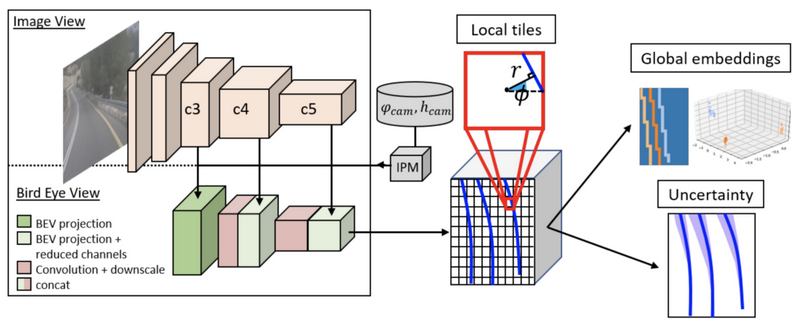
\includegraphics[width=0.8\linewidth, height=4cm]{images/3DLaneNET++.png} 
\label{fig:subim1}
%\end{subfigure}

\caption{Semi-local 3D LaneNet pipeline \footcite{DBLP:journals/corr/abs-2011-01535} }
\label{fig:image2}
\end{figure}
\end{frame}
%%%%%%%%%%%%%%%%%%%%%%%%%%%%%%%%
\begin{frame}{Pros and Cons of Previous Work (1/2)}
    \textbf{Gen-LaneNet}
    
    \begin{itemize}
        \item Dual stage pipeline is flexible in terms of replacing the first stage by better 2D lane detection algorithms. 
        \item Lane detection and prediction of 3D geometry are treated as different tasks. 
        \item Introduced a generalized virtual top view for the correction of points in top view when a ego vehicle moves uphill or downhill.
        \item Can not handle different topologies when the lane lines are perpendicular to the ego vehicle.
        \item Can not generalize well with different cameras.
    \end{itemize}

\end{frame}

%%%%%%%%%%%%%%%%%%%%%%%%%
\begin{frame}{Pros and Cons of Previous Work (2/2)}
    \textbf{Semi-local 3D LaneNet}
    \begin{itemize}
        \item Prediction of 3D lane lines are done semi-locally and in an anchor-less manner. 
        \item BEV mask is broken into tiles and each tile is responsible for contributing one point to lane curve.
        \item Can generalize well to different topologies.
    \end{itemize}


\textbf{Takeaway}
\begin{itemize}
    \item We combine the effectiveness of dual stage pipeline proposed by Gen-LaneNet and semi-local anchor-less representation of the 3D lane curves  
\end{itemize}
\end{frame}

%%%%%%%%%%%%%%%%%%%%%%%%%%%
\begin{frame}{Proposed Dual Stage Semi-local Anchor-less 3D Lane Detector}


 \begin{figure}[H]
     \centering
     
%\begin{subfigure}{\textwidth}
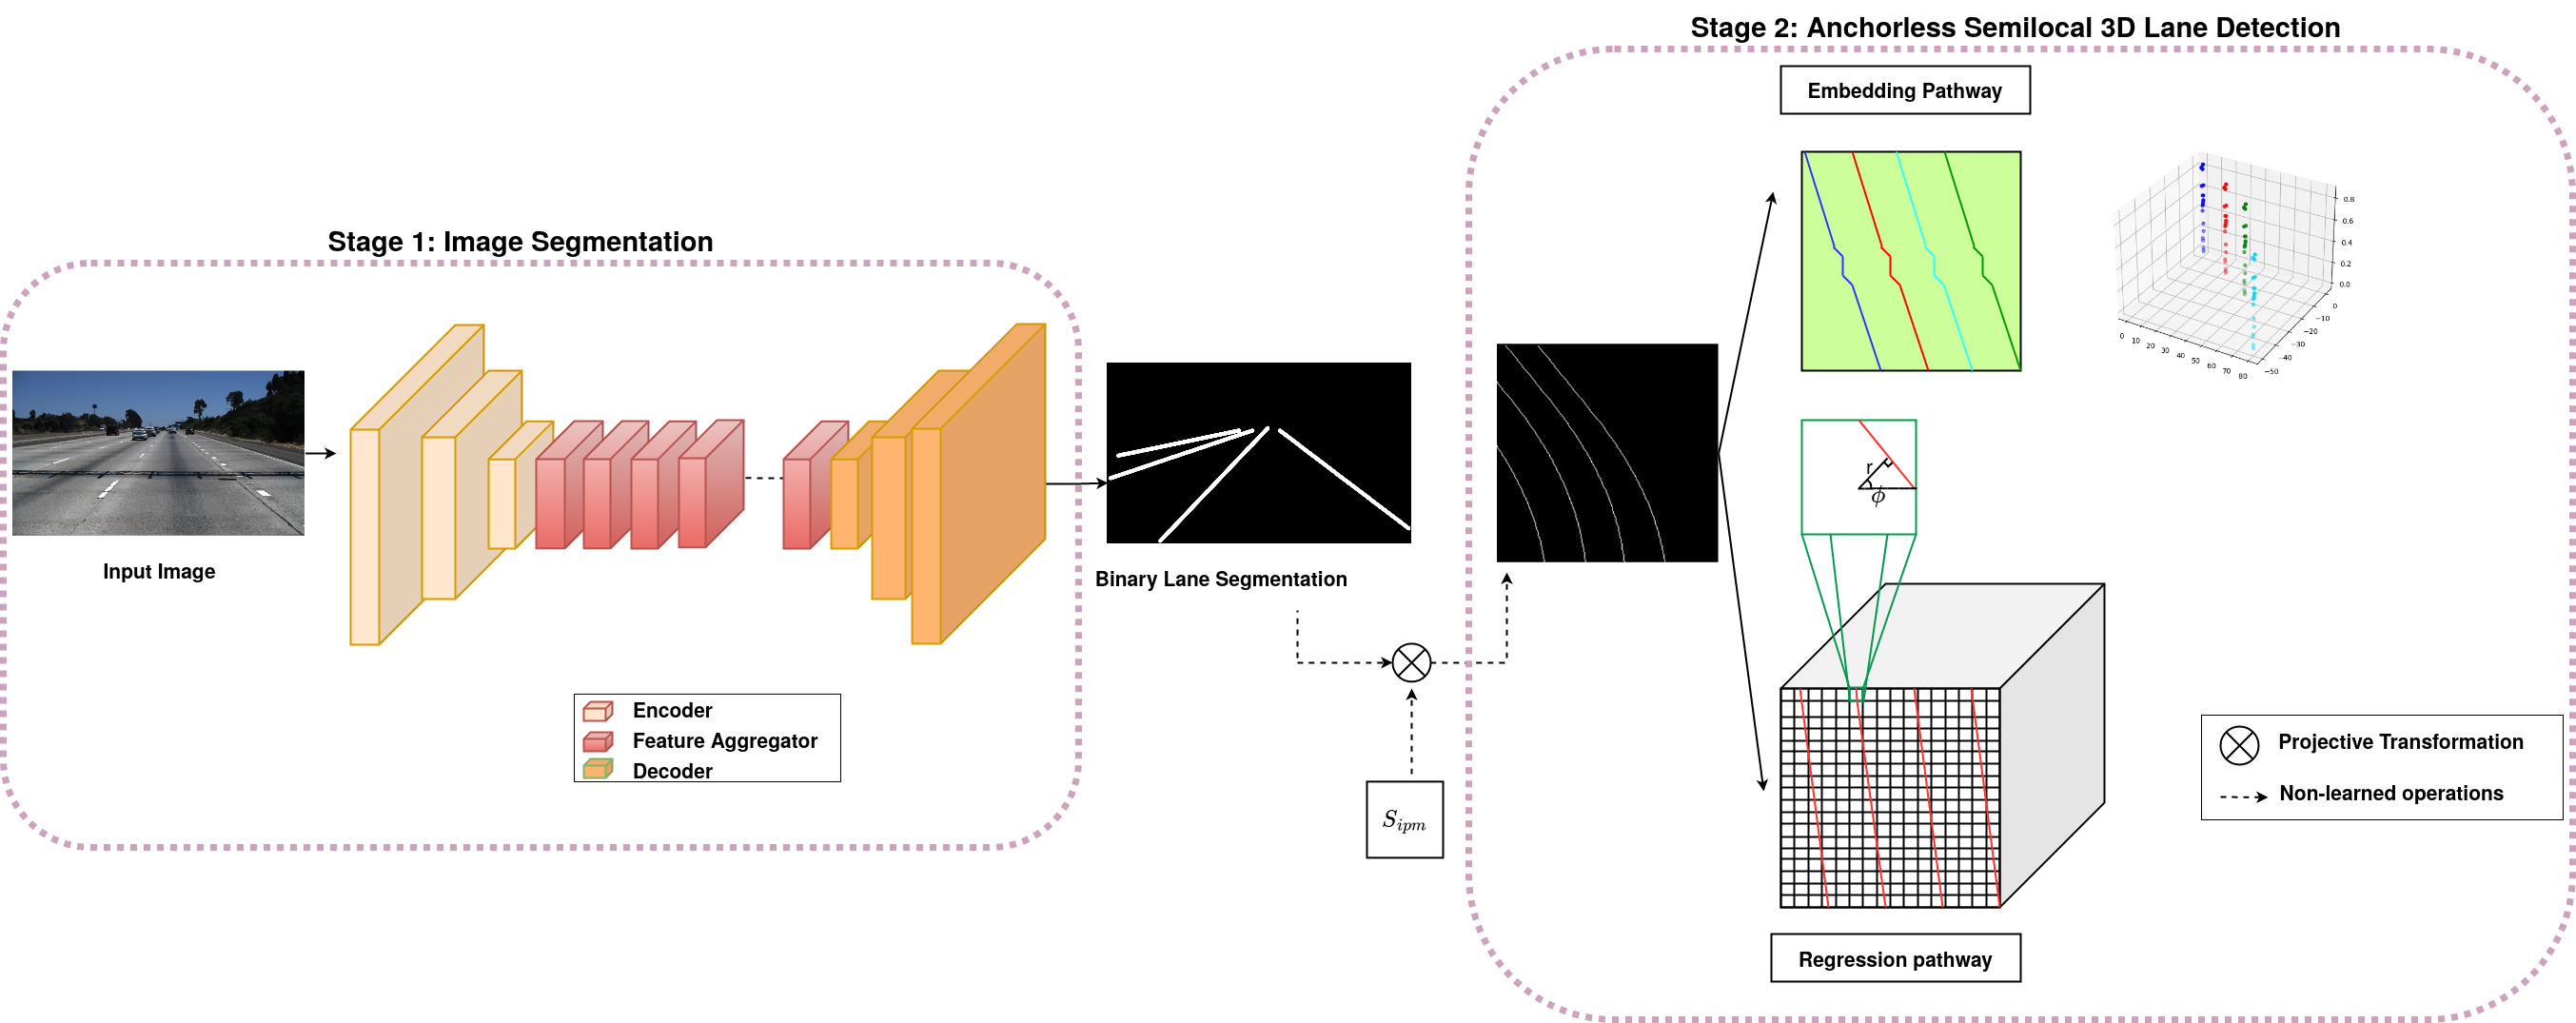
\includegraphics[width=0.8\linewidth, height=4.5cm]{images/3DlaneAUXNet.png} 
\label{fig:subim1}
%\end{subfigure}

\caption{Dual stage semi-local anchor-less 3D lane detection pipeline }
\label{fig:image2}
\end{figure}
\end{frame}

%%%%%%%%%%%%%%%%%%%%%%%%%%%%%%%%%%%%
%% Stage 1: Binary Lane Segmentation
%% s-1 DIAG... of pipeline 
%% s-2 mention why increased efficated RESNET ---- >  SCNN, RESA ---> decoders
%% s-3 Traning details and datasets used
%% s-4 Training Targets and Loss functions used
%% s-5 QA and EMP Results with cross entropy
%% s-6 QA and EMP Results after task loss balancing 
%% s-7 QA and EMP Results with combined GenLaneNet 



\begin{frame}
\printbibliography
\end{frame}
\end{document}
